\chapter{Searching for Long Lived Particles}
\label{chap:llps}

A particle is \emph{long lived} if the distance it travels before decaying can be discerned by the detector.  This is contrasted with a promptly decaying particle whose decay products point back to the collision point. In \ac{ATLAS}, \acp{LLP} are generally those with a lifetime of more than 1.5 ps (longer than that of a b-hadron) and travel more than 1 mm before decaying.

A \ac{LLP} can decay somewhere inside of the detector or it can pass through the detector without decaying. Note that a detector-stable particle does not necessarily imply a truly stable particle; for example, muons are detector-stable because they never decay within the detector volume. Prompt searches can be used look for neutral stable particles, like dark matter candidates, by calculating \ac{MET} from the prompt particles. \ac{LLP} searches either look directly for the signature of the particle, or look for the products of the metastable decay. This brings technical challenges because standard particle identification algorithms and analysis techniques are not designed for these signatures. It also provides a way to probe processes with extremely small cross sections due to the lack of \ac{SM} processes with the same final state.

This chapter gives an overview of fundamental concepts for \ac{LLP} searches at colliders.

\section{Lifetime}
%USED theory-llp-whitepaper.pdf
An individual particle's lifetime cannot be predicted theoretically, but the distribution of lifetimes of a sample of the same particle can be determined from its probability of decay per unit time or \emph{width}, $\Gamma$:

\begin{equation}
\Gamma = \frac{1}{2m_{X}} \int d\Pi_f \big| \mathcal{M}(m_X \rightarrow \{p_f\})\big|^2
\end{equation}
where $m_X$ is the mass of the particle, $\mathcal{M}$ is the matrix element for the particle's decay into its decay products $\{p_f\}$ and $d\Pi_f$ is the Lorentz-invariant phase space of the decay.
If particle can decay in several different ways, the width of each decay various channel is summed to calculated the particle's \emph{total width}. The branching ratio of a particle decaying via a process $i$ is given as
\begin{equation}
\text{Br}_{i} = \frac{\Gamma_{i}}{\Gamma_{\text{total}}}
\end{equation}

$\text{Br}_{i}$ gives the probability that a particle will decay via process $i$. This is different than the cross section, which measures the probability for a scattering process to result in a given final state. The width is referred to as such because in an experiment with negligible statistical and systematic uncertainties, the width is the full-width-at-half-max of the Gaussian peak of the particle mass spectrum, sketched in \autoref{fig:width}. 

\begin{figure}[!h]
\centering
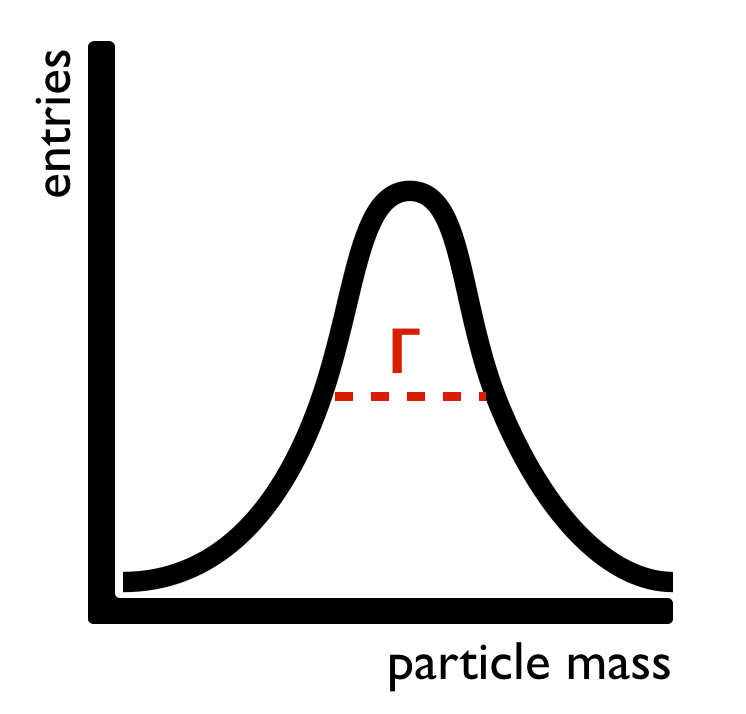
\includegraphics[width=.3\textwidth]{figures/theory/particle-width.png}
\caption{A sketch of a particle mass histogram. The width is shown in red.}
\label{fig:width}
\end{figure}

In the sample of particles, the number of particles $N$ that exist at a time $t$ decreases exponentially from the initial number of particles $N(0)$:

\begin{equation}
N(t) = N(0) e^{-\Gamma t}
\end{equation}

A particle's ``lifetime'', $\tau$, is defined as the time it takes for $\frac{1}{e}$ of the population of particles to decay:
\begin{equation}
\tau = \frac{1}{\Gamma}
\end{equation}
 
In order for the lifetime of a particle to be long, the width must be small, meaning that the matrix element or allowed phase space must be small. A small matrix element can be caused by a small coupling, or very off-shell intermediate states (like a neutron). A small phase space can be caused by almost-degenerate mass spectra (like a muon). All of these scenarios are common in both the \ac{SM} and many \ac{BSM} theories. The range of lifetimes of selected \ac{SM} particles can be seen in \autoref{fig:llp-mass-lifetime} \cite{llp-whitepaper}


\begin{figure}[!h]
\centering
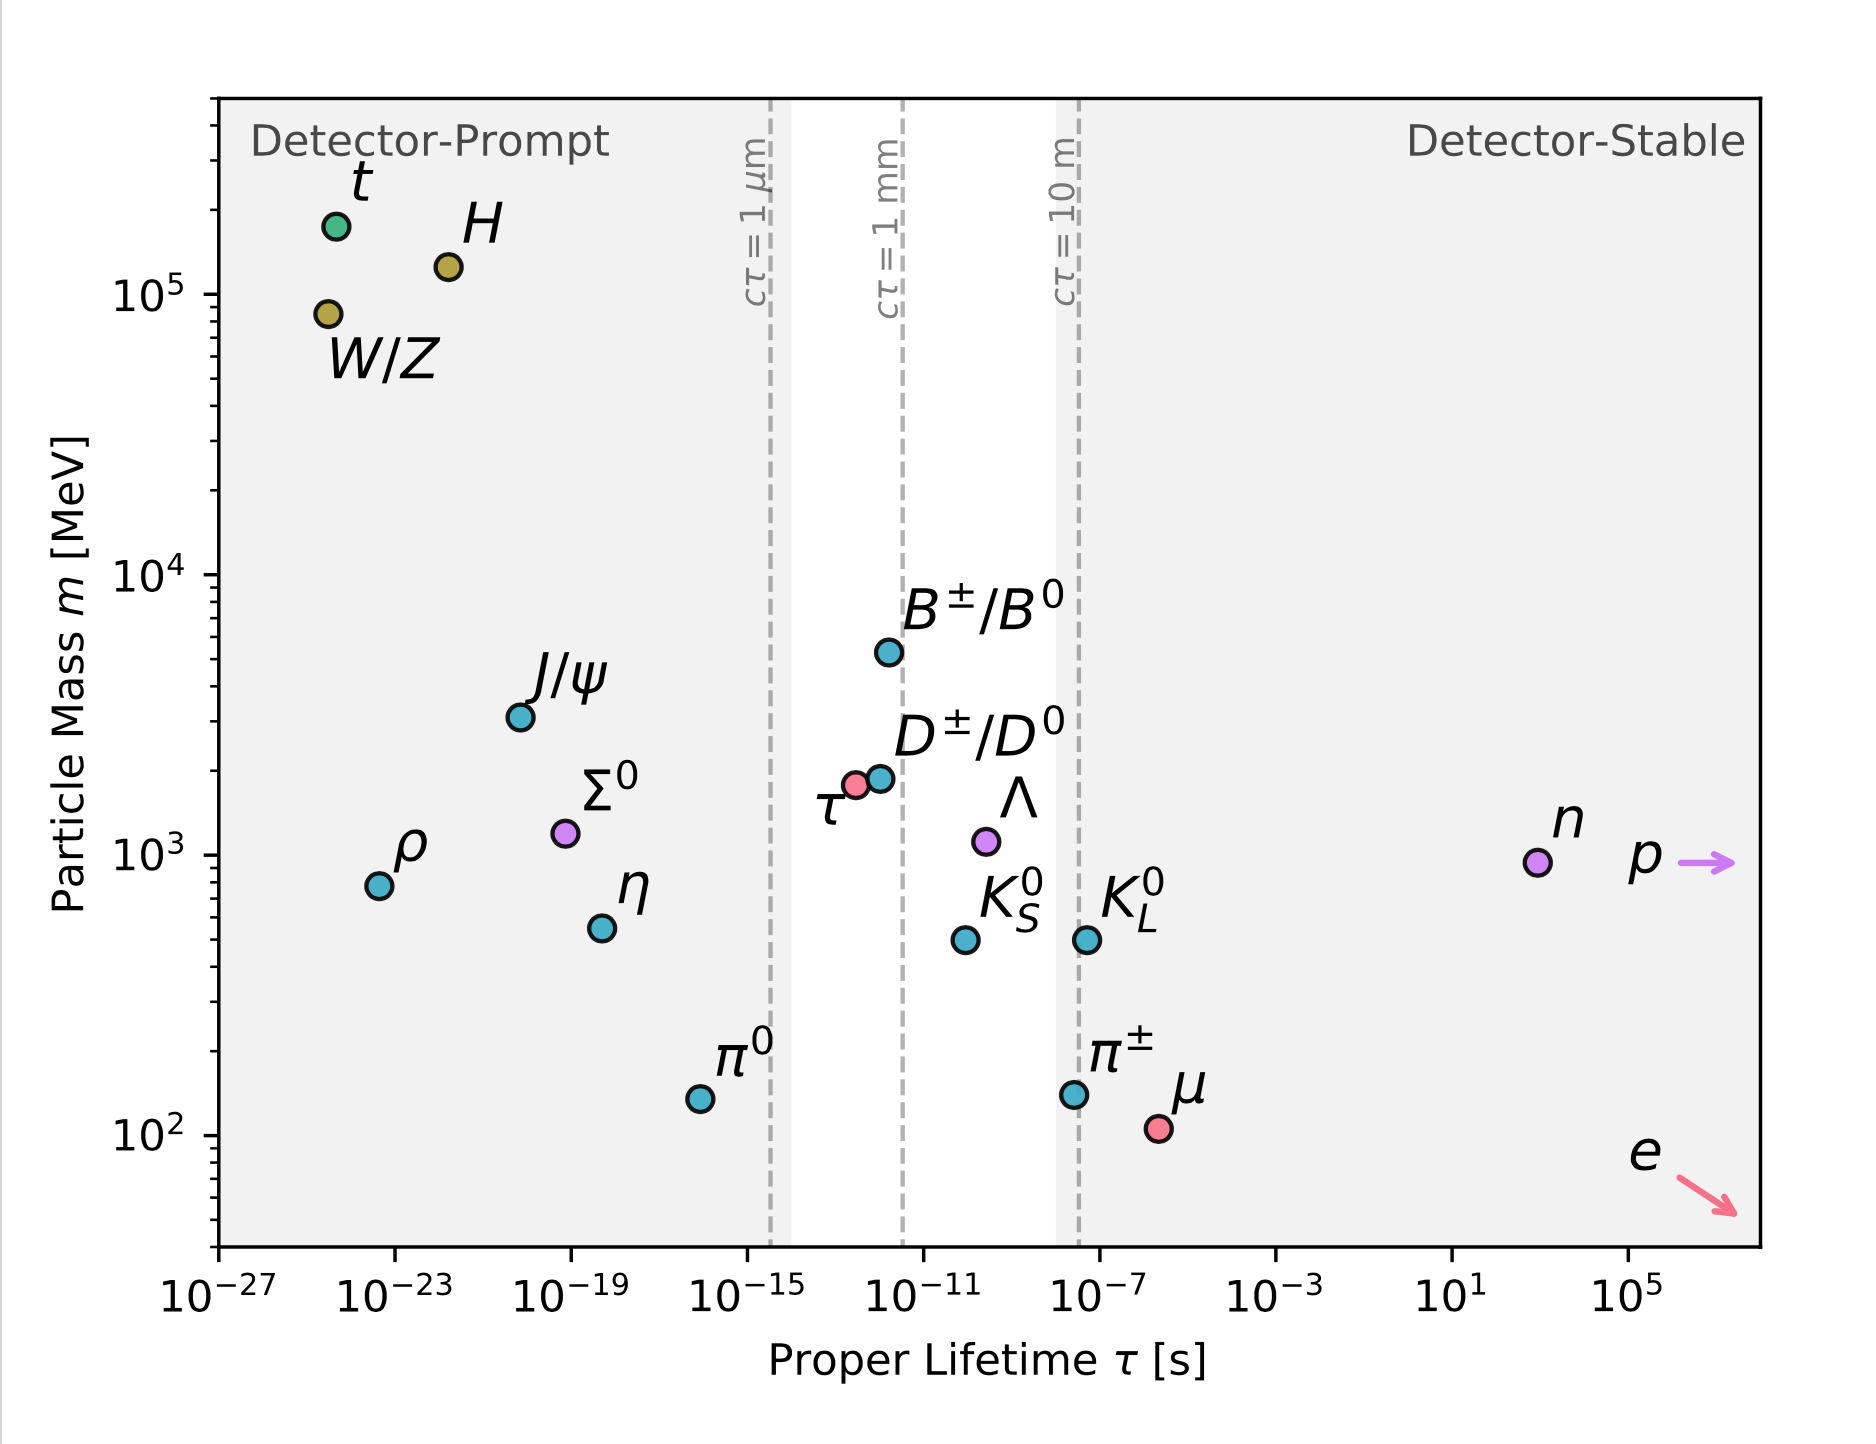
\includegraphics[width=.6\textwidth]{figures/theory/LLP-mass-lifetime.png}
\caption{A mass and proper lifetime distribution of particles in the \ac{SM}. There is a wide range of both masses and lifetimes. Shaded regions indicate detector-prompt or detector-stable particles. This assumes that particles traveling at the speed of light $\beta = 1$. \cite{llp-whitepaper}}
\label{fig:llp-mass-lifetime}
\end{figure}

\section{Particle Decays}
%USED theory-LLP-Banerjee.pdf

The distance traveled by any relativistic particle can be described by
\begin{equation}
d = \beta \gamma t
\label{eq:sr_d}
\end{equation}
where $\gamma$ and $\beta$ have the usual special relativistic definitions: $\gamma = E/m = (1-\beta^2)^{(-\frac{1}{2})}$, $\beta = v/c = |\vec{p}|/E$, $v$ is the particle's velocity, $t$ is the time during which the particle moves, and $c$ is the speed of light. In the laboratory frame, the distance the particle travels before decaying is given by sending $t \rightarrow \tau_{0}$ in \autoref{eq:sr_d}, where $\tau_{0}$ denotes the proper lifetime of the particle measured in its own rest frame.

There is an exponential probability that the particle will decay at a given time ($t$), given by 
\begin{equation}
P(t) = e ^{-t/(\gamma \tau)}
\end{equation}
A particle with a large $\tau$ has a wider probability distribution and there is a larger range of times in which the particle can decay. Practically, this means that a wide variety of signatures are possible from the same theoretical particle with large $\tau$: it can decay promptly, somewhere inside of the detector volume, or be detector-stable.


\section{\label{sec:llp-searches}Searches}

Many searches are done by both \ac{ATLAS} and \ac{CMS} to target a variety of possible detector signatures. There are two primary ways that this is achieved: \emph{direct searches} for the \ac{LLP} itself or \emph{indirect searches} for its decay products. A sketch of a different \ac{LLP} signatures is shown in \autoref{fig:llp-signatures} 

\begin{figure}[!h]
\centering
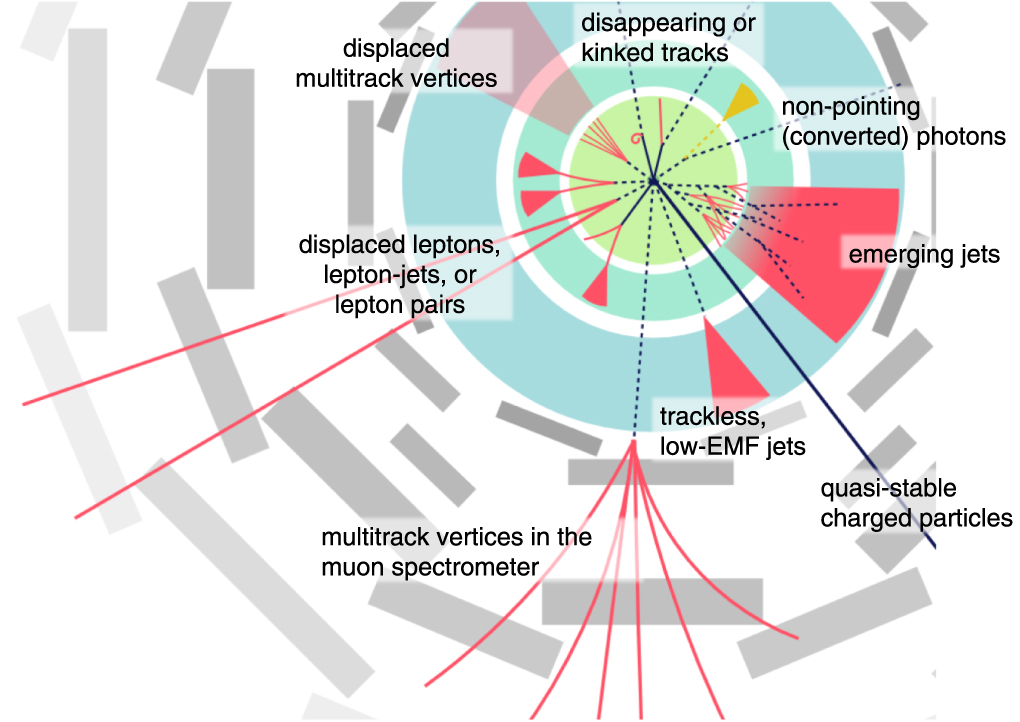
\includegraphics[width=.8\textwidth]{figures/theory/llp-signatures.jpg}
\caption{A sketch of a sample of different \ac{LLP} signatures in the \ac{ATLAS} detector. \cite{llpdiagram}}
\label{fig:llp-signatures}
\end{figure}


\paragraph{Direct searches} 

If a particle is very massive and charged, \ac{LLP} interaction with the detector could be observed. Searches are performed looking for tracks have high ionization energy loss in the Pixel detector, indicating a very heavy particle traversing the \ac{ID} \cite{SUSY-2014-09}. Searches for slow moving, heavy stable particles are performed by looking for highly ionizing tracks in the \ac{ID} that match tracks in the \ac{MS} \cite{SUSY-2016-02}. Other searches look for a \ac{LLP} that decays into invisible particles by looking for short, disappearing tracks \cite{SUSY-2016-06, CMS-EXO-16-044}. These signatures generally involve prompt tracks

\paragraph{Indirect Searches} 

If more than one of the products of the \ac{LLP} decay are visible to the detector, one can look for its decay vertex. The \ac{LLP} will travel some distance from the \ac{PV}, where the particle is produced, and its decay vertex will be displaced, called a \ac{DV}. In this case, direct information about $\tau_{0}$ of the particle can be deduced from the difference in distance between the \ac{LLP}'s production and decay vertices. This vertices can appear in either tracking volume of the detector (\ac{ID} or \ac{MS}). There are many searches for \ac{DV}s in \ac{ATLAS}, many in conjunction with other physics objects like leptons, jets, or \ac{MET} depending on the particular theory model being probed \cite{dvplusmu,SUSY-2016-06,SUSY-2014-02,CMS-EXO-18-007,CMS-EXO-17-018,CMS-SUS-14-020}. 

One can also look for the decay products of the \ac{LLP} without a \ac{DV} via unconventionally presenting physics objects. Examples include photons that do not point back to the \ac{PV} in the \ac{EM} calorimeter \cite{SUSY-2013-17}, or emerging jets, which become visible midway through their hadronization \cite{CMS-EXO-18-001}. In this analysis, the target signature is leptons whose trajectories do not point back to the \ac{PV}.

For indirect searches, it is often convenient to use \dzero, the transverse impact parameter, as a measure of particle displacement. The \dzero is a parameter of \ac{ID} track fit, discussed in \autoref{sec:trackreco}. It does not give direct information about $\tau_{0}$, but it can be known with high precision. The distance the particle traveled from the collision, $R$, would give direct information about the proper lifetime of the particle, but the detector can only provide the radius of the first \ac{ID} hit in the track. The distance between silicon \ac{ID} layers at minimum 30 mm and any requirements on $R$ are very sensitive to transient detector failures. \dz, however, has a $\mathcal{O}(10~\mu \textrm{m})$ resolution, shown in \autoref{fig:trking_d0_res}. The \dz of the decay products of a \ac{LLP} with a longer lifetime have wider \dzero distributions as seen in \autoref{fig:d0-rltns}. The \dz of the decay products is also correlated with the momentum of the \ac{LLP}, shown in \autoref{fig:d0-pt}. This relationship induces a correlation between the \pt and \dz of the decay products.

\begin{figure}[!h]
\centering
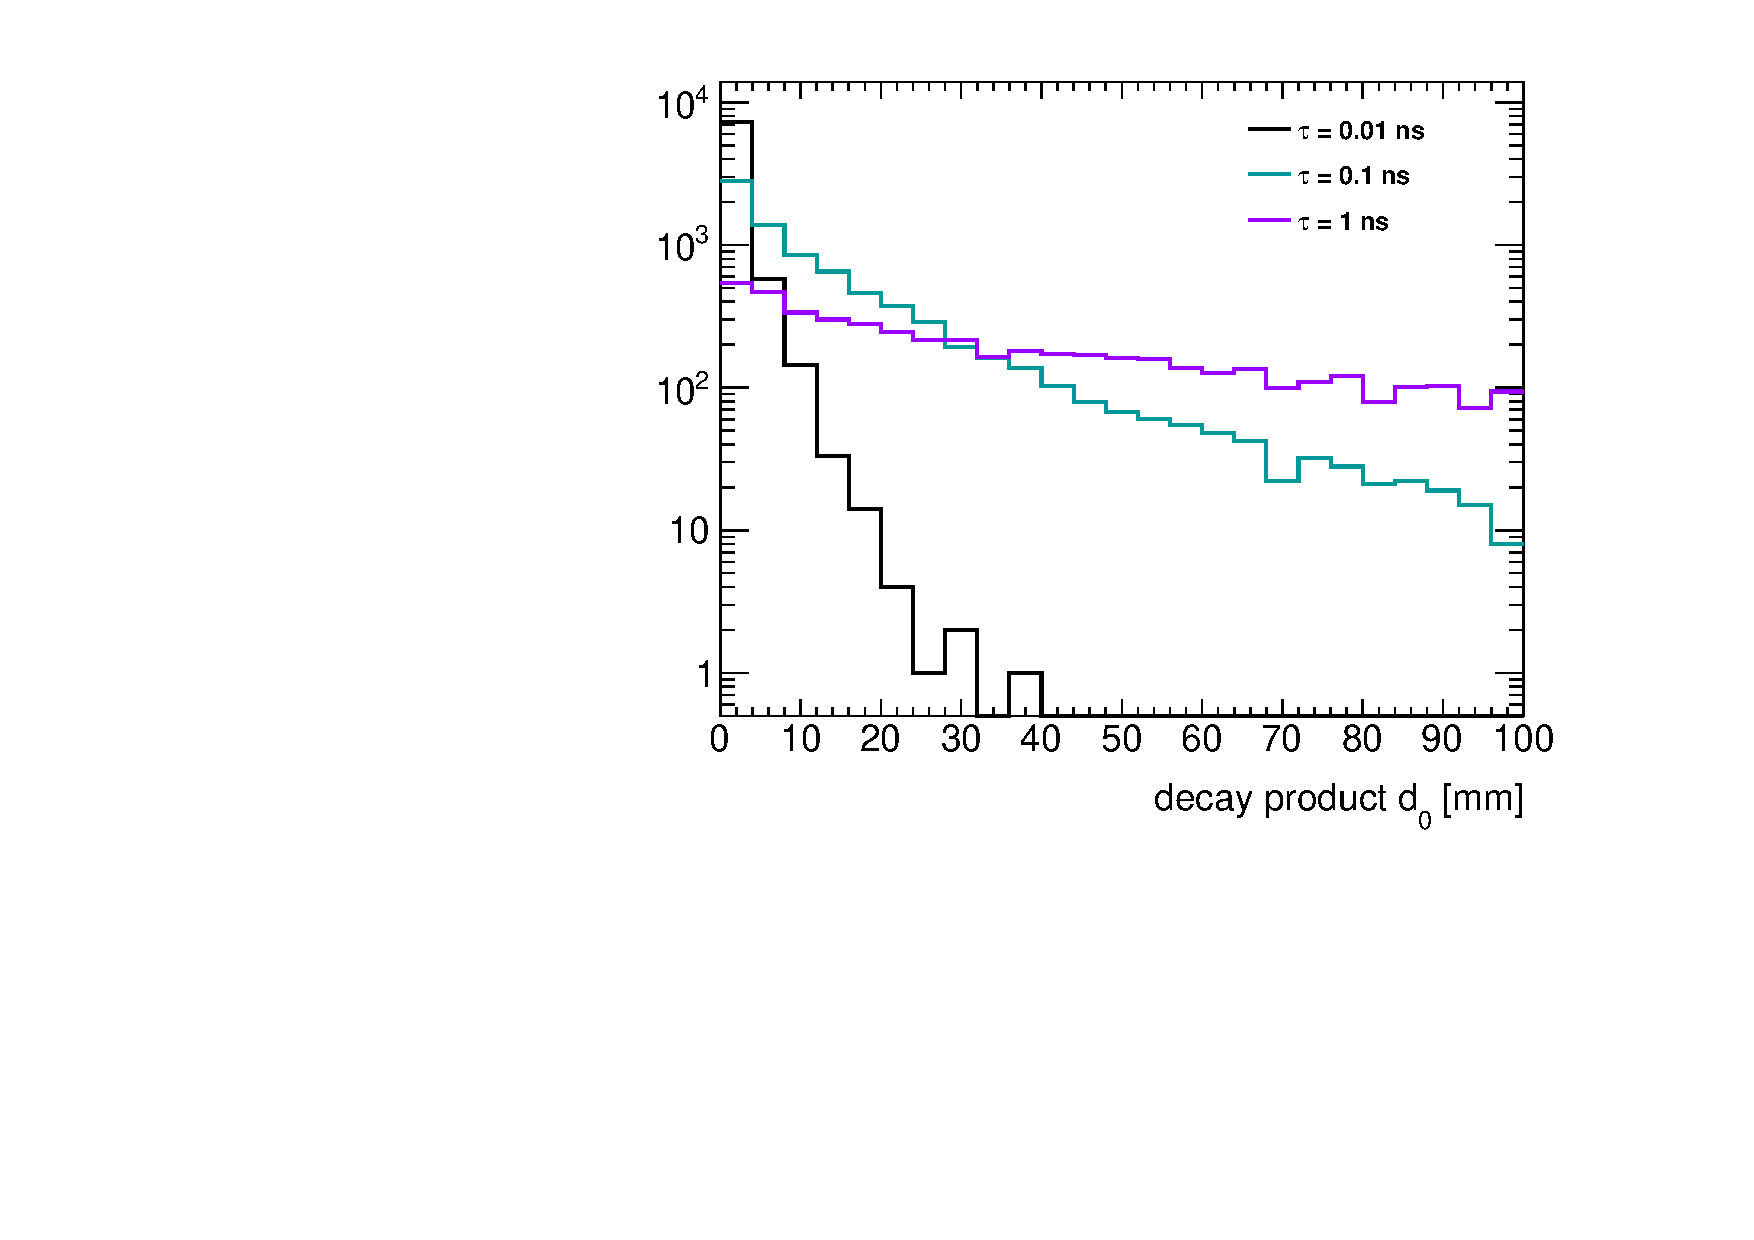
\includegraphics[width=.48\textwidth]{figures/theory/signal_d0.pdf}
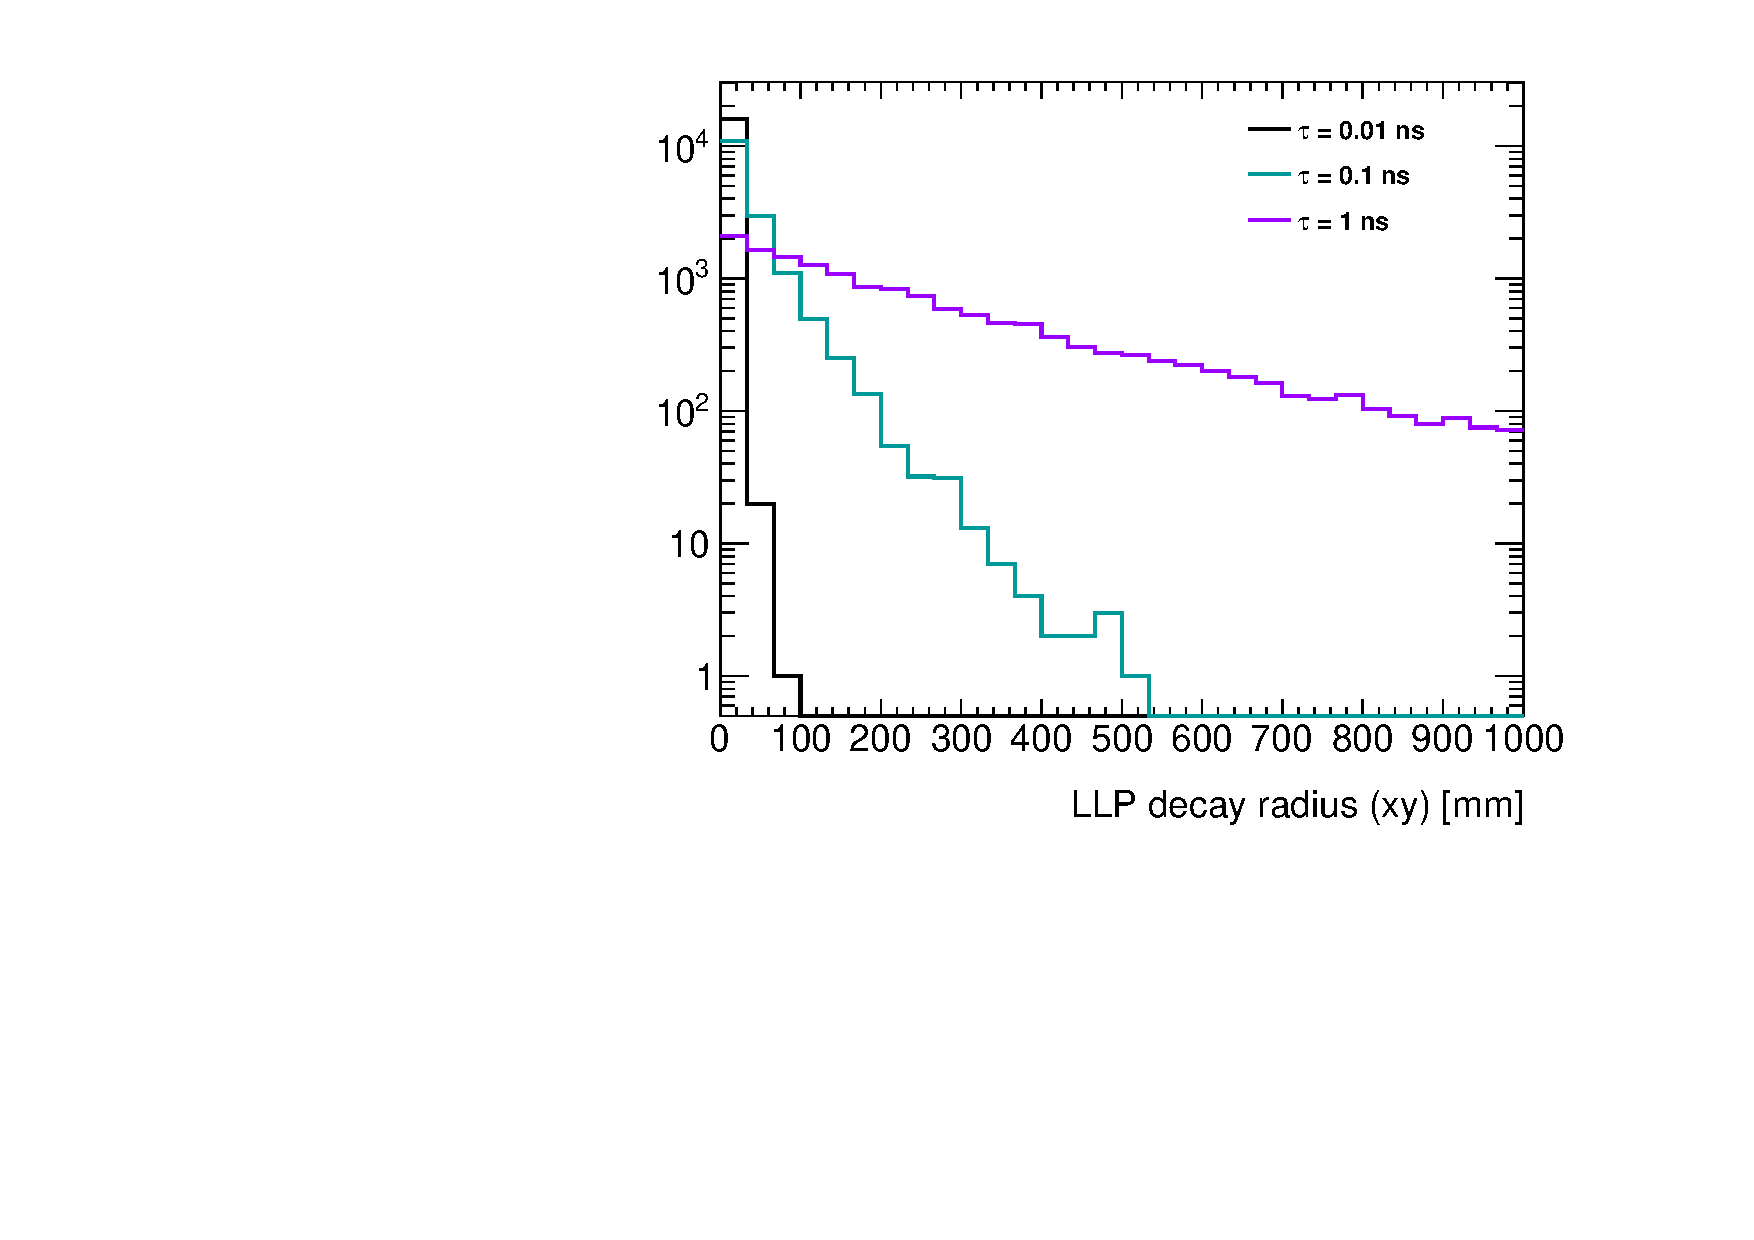
\includegraphics[width=.48\textwidth]{figures/theory/signal_rxy.pdf}
\caption{\dzero (left) and transverse decay radius ($x-y$) of \ac{LLP}s with different $\tau$. The left plot demonstrates that while \dzero does not directly give information about $\tau$, decay products of particles with longer lifetimes have wider \dzero distributions. These plots are made at truth level.}
\label{fig:d0-rltns}
\end{figure}

\begin{figure}[!h]
\centering
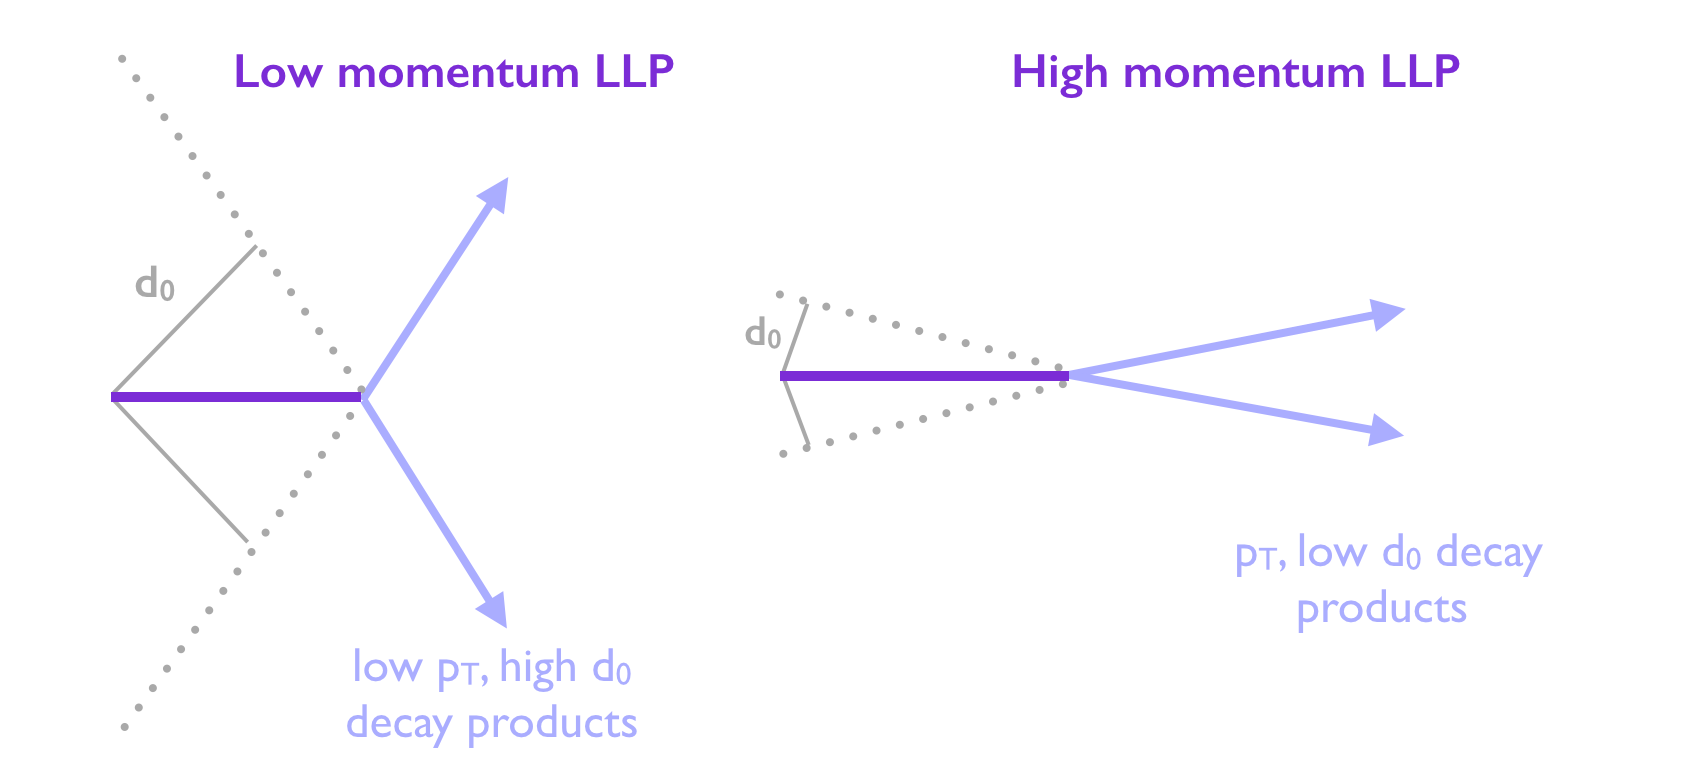
\includegraphics[width=.6\textwidth]{figures/theory/pt-d0.png}
\caption{A sketch of the relationship between the momentum of the parent \ac{LLP} and the \dz of the daughter particles.}
\label{fig:d0-pt}
\end{figure}

\subsection{Common Strategies}

Due to the technical challenges associated with \ac{LLP} searches, analyzers want their result to be applicable to as many potential \ac{BSM} particles as possible and they aim to make their selections as \emph{model-independent} as possible. This means that, while there is usually a model to which a search brings unique sensitivity, the search not over-optimized for this model. For example, in this analysis, the events are only required to have two displaced leptons. The slepton decays in the \ac{GMSB} \ac{SUSY} model include \ac{MET} from the gravitino, but no requirement is made to ensure the result is sensitive to other possible models that might not include \ac{MET}.


\todo{if there's time: implications of 0 background search, why are 3 events required for discovery? -- I found a paper but this will take me a while to digest}


